\documentclass[12pt]{llncs}
%\usepackage{sbc-template}
\usepackage{graphicx,url}

%\usepackage[brazil]{babel}   
\usepackage[latin1]{inputenc}  
\usepackage{amsfonts}
\usepackage{amsmath}
\usepackage{subfigure}
     
%\sloppy

%\pdfpagewidth=8.5truein
%\pdfpageheight=11truein

% Equation terms definition
\newcommand{\route}[1]{\ensuremath{P_#1}}	%route for driver 'i'
\newcommand{\optRoute}[1]{\ensuremath{P_#1^*}}	%optimal route for driver 'i'

\newcommand{\travTime}{\ensuremath{t_l}} 	%travel time on link 'l'
\newcommand{\fftt}{\ensuremath{f_l}} 		%free-flow travel time of link 'l'
\newcommand{\linkCap}{\ensuremath{c_l}}		%capacity of link 'l'
\newcommand{\veh}{\ensuremath{v}}		%number of vehicles

\newcommand{\ett}[1]{\ensuremath{e_#1}}		%estimated travel time for agent 'i'
\newcommand{\expVeh}{\ensuremath{v_e}}		%estimated number of vehicles

\newcommand{\att}[1]{\ensuremath{a_#1}}		%actual travel time for driver 'i' on route P

\newcommand{\reward}[1][]{\ensuremath{R_#1}}	%reward

\newcommand{\congRoads}{\ensuremath{C}}		%the set of congested roads
\newcommand{\numCong}{\ensuremath{n}}		%number of congested roads
\newcommand{\overLoadFactor}{\ensuremath{o}}	%overload factor - measures severity of congestions

\title{Reinforcement learning for route choice in an abstract traffic scenario}


\author{
  Anderson R. Tavares\inst{1} \and Ana L. C. Bazzan\inst{1}
}

\institute{Instituto de Inform\'atica -- Universidade Federal do Rio Grande do Sul
  (UFRGS)\\
  Caixa Postal 15.064 -- 91.501-970 -- Porto Alegre -- RS -- Brazil
  \email{\{artavares,bazzan\}@inf.ufrgs.br}
}

\begin{document}

\maketitle

\begin{abstract}
Traffic movement in a commuting scenario is a phenomena that emerges from individual and uncoordinated route choice by drivers. Every driver wishes to achieve reasonable travel times from his origin to his destination and, from a global point of view, it is desirable that the load gets distributed proportionally to the roads capacity on the network. This work presents a reinforcement learning algorithm for route choice which relies solely on drivers experience to guide their decisions. Experimental results demonstrate that reasonable travel times can be achieved and vehicles distribute themselves over the road network avoiding congestion. The proposed algorithm makes use of no coordinated learning mechanism, making this work is a case of use of independent learners concept.
\end{abstract}


%\category{I.2.11}{Artificial Intelligence}{Distributed Artificial Intelligence}[Multiagent Systems]

%\terms{Algorithms}

%\keywords{Multiagent reinforcement learning, multiagent systems, traffic assignment}

\section{Introduction}
\label{sec:intro}

The subject of traffic and mobility presents challenging issues to authorities, traffic engineers and researchers. To deal with the increasing demand, techniques and methods to optimize the existing road traffic network are attractive since they do not include expensive and environmental-impacting changes on infrastructure.

In a commuting scenario, it is reasonable to assume that drivers choose their routes independently and, most of the time, uninformed about real-time road traffic condition, thus relying on their own experience. Daily commuters usually have an expectation on the time needed to arrive on their destinations and, if a driver reaches its destination within expectation, his travel time can be considered  reasonable. From a global point of view, it is desired that vehicles gets distributed on the road network proportionally to the capacity of each road. Multiagent systems like this commuting scenario, where each agent tries to maximize its own utility function, while at the same time there is an global utility which rates the whole system's behavior are called collectives. The local and global goals can be highly conflicting and there is no general approach to tackle this complex question of collectives, as shown on \cite{Tumer&Wolpert2004}.

Traffic assignment deals with route choice between origin-destination pairs in transportation networks. In this work, traffic assignment will be modeled as a reinforcement learning problem. This approach uses no communication among drivers and makes no unrealistic assumptions such as the drivers having complete knowledge on real-time road traffic condition. In reinforcement learning problems, agents make decisions using only their own experience which is gained through interaction with the environment.

The scenario studied in this work abstracts some real-world characteristics such as vehicle movement along the roads, allowing us to focus on the main subject which is the choice of one route among the several available for each driver.

The remainder of this document is organized as follows: Section \ref{sec:concepts} presents basic traffic engineering, single and multiagent reinforcement learning concepts that will be used throughout this paper. Section \ref{sec:related} presents and discusses related work done in this field. Section \ref{sec:proposal} presents the reinforcement learning for route choice algorithm whose results are discussed in Section \ref{sec:results}. Finally, Section \ref{sec:conclusions} concludes the paper and presents opportunities for further study.

\section{Concepts}
\label{sec:concepts}
\subsection{Commuting and traffic flow}

A road network can be modeled as a set of nodes, which represent the intersections, and links among these nodes, which represent the roads. The weight of a link represents a form of cost associated with the link. For instance, the cost can be the travel time, fuel spent or distance.

A subset of the nodes contains the origins of the road network, where drivers start their trips, and another subset represents the destinations, where drivers finish their trips. In a commuting scenario, a driver's trip consists on a set of links, forming a route between his origin and destination (OD pair) among the available routes.

Traffic flow is defined by the number of entities that use a network link in a given period of time. Capacity is understood as the number of traffic units that a link supports in a given instant of time. Load is understood as the demand generated on a link at a given moment. When demand reaches the link's maximum capacity, the congestion is formed.

Traffic assignment methods that consider congestion effects in urban settings needs a suitable cost function that relates link's attributes (capacity, free-flow travel time) and traffic flow on the entire road network. However, a simplified form that relates attributes of a  given link and traffic flow only on that link can be used, although with some loss of realism. One of the most common function of this type is shown on Eq. \eqref{eq:tt} \cite{Ortuzar&Willumsen2001}.

\begin{equation}
\label{eq:tt}
\travTime(\veh) = \fftt[1 + \tau \left(\frac{\veh}{\linkCap}\right)^\beta]
\end{equation}

In this function, $\travTime$ is the travel time on link $l$, $\linkCap$ is the link's capacity, $\fftt$ is the free-flow travel time on link $l$ and $\tau$ and $\beta$ are calibration parameters. This will be the travel time function used throughout the present work.

\subsection{Reinforcement Learning}

Reinforcement learning (RL) deals with the problem of making an agent learn a behavior by interaction with the environment. The agent perceives the environment state, chooses an action available on that state, and then receive a reinforcement signal from the environment. This signal is related to the new state reached by the agent. The agent's goal is to increase the long-run sum of the reinforcement signals received \cite{Kaelbling+1996}.

Usually, a reinforcement learning problem is modeled as a Markov Decision Process (MDP), which consists of a discrete set of environment states $(S)$, a discrete set of actions $(A)$, a state transition function ($T: S \times A \to \Pi(S))$, where $\Pi(S)$ is a probability distribution over S) and a reward function $(R: S \times A \to \mathbb{R})$. $T(s, a, s')$ means the probability to go from state $s$ to $s'$ after performing action $a$ in $s$.

The optimal value of a state, $V^*(s)$, is the expected infinite discounted sum of rewards that the agent gains by starting at state $s$ and following the optimal policy. A policy $(\pi)$ maps the current environment state $s \in S$ to an action $a \in A$ to be performed by the agent. The optimal policy $(\pi^*)$ represents the mapping from states to actions which maximizes the future reward.

For the next sections it will be assumed that the reader is familiar with Q-learning. For more information about Q-learning, the reader may refer to \cite{Watkins&Dayan1992}.

\subsection{Multiagent Reinforcement Learning}
A multiagent system can be understood as group of agents that interact with each other besides perceiving and acting in the environment they are situated. The behavior of these agents can be designed a priori. In some scenarios this is a difficult task or this pre-programmed behavior is undesired, so that the adoption of learning (or adapting) agents is a feasible alternative \cite{Busoniu+2008}.

For the single-agent reinforcement learning task, consistent algorithms with good convergence are known. When it comes to multiagent systems, several challenges arise. Each agent must adapt itself to the environment and to the other agents behaviors. This adaptation demands other agents to adapt themselves, changing their behaviors, thus demanding the first to adapt again. This nonstationarity turns the convergence properties of single-agent RL algorithms invalid.

Single-agent RL tasks modeled as a MDP already have scalability issues on realistic problem sizes and these issues gets worse for multi agent reinforcement learning (MARL). For this reason, some MARL tasks are tackled by making each agent learn without considering other agents adaptation. In this situation, one agent understands other agents learning and changing their behavior as a change of environment dynamics. In this approach, the agents follow the concept of independent learners \cite{Claus&Boutilier1998}. It is demonstrated in \cite{Claus&Boutilier1998} that in this case, Q-learning is not as robust as it is in single-agent settings. Also, it is remarked by \cite{Littman1994} that training adaptive agents without considering other agents adaptation is not mathematically justified and it is prone to reaching a local maximum where agents quickly stop learning. Even so, some researchers achieved amazing results with this approach.

\section{Related work}
\label{sec:related}

In traffic engineering, \cite{Bazzan&Kluegl2007} remarks that traditional methods for route assignment assume that users of transportation systems are perfectly rational. These traditional methods do not consider individual behavior, atributes and decision-making processes. More than that, the ability of dealing with incomplete information and adapting to changes on the environment are not regarded on traditional methods.

Agent-based simulation support dealing with dynamic environments, incomplete information and modeling of agent's adaptation to the environment, individual behavior, atributes and decision-making processes. Application of intelligent agent architectures to route choice is present on a number of publications. Next, some works based on this agent-based approach are reviewed.

Several works, like \cite{Bazzan+2000icmas, Chmura&Pitz2007, Kluegl&Bazzan2004}, use abstract scenarios, most of the times inspired by congestion or minority games. On these scenarios, agents have to decide between two routes and receive a reward based on the occupancy of the chosen route. This process is repeated and there is a learning or adaptation mechanism that guides the next choice based on previous rewards.

With this process, a Pareto-efficient distribution or the Wardrop's equilibrium \cite{Wardrop1952} may be reached. In this condition, no agent can reduce its costs by switching routes without rising costs for other agents. 

Two-route scenarios are studied in \cite{Bazzan+2000icmas, Chmura&Pitz2007, Kluegl&Bazzan2004}. The former analyses the effect of different strategies on minority game for binary route choice. The second uses a reinforcement learning scheme to reproduce human decision-making in a corresponding experimental study. The third includes a forecast phase for letting agents know the decision of the others and then let they change their original decision or not. Each one of these works assessed relevant aspects of agents decision-making process, even though only binary route choice scenarios were studied. The interest on the present work is to evaluate a route choice algorithm in a more complex scenario, with several available routes.

This kind of complex scenario was investigated by \cite{Bazzan&Kluegl2008}. On their work, Bazzan and Kl\"ugl assessed the effect of real time information on drivers' route replanning, including studies with adaptive traffic lights. In the most successful route replanning strategy presented on that work, the authors assume that the entire network occupancy is known by the drivers. This assumption was needed for assessing the effects of re-routing, although the availability of real time information of the entire network for all the drivers is an unrealistic assumption.

More recently, the minority game algorithm was modified for use in a complex scenario with several available routes \cite{Galib&Moser2011}. Using the proposed algorithm, drivers achieve reasonable (within expectation) travel times and distribute themselves over the road network in a way that few roads get overused. The modified minority game algorithm uses historic usage data of all roads to choose the next one on the route. Having historical information of the roads used by the driver is a reasonable assumption, but having historic information of all roads on the network is unrealistic. The algorithm proposed on the present work will be compared with the modified minority game. 

\section{Algorithm and scenario}
\label{sec:proposal}

\subsection{Reinforcement learning for route choice}

In this study, one agent will consider the others as part of the environment, following the concept of independent learners. Prior to the present work, independent learning agents were studied in cooperative repeated games \cite{Claus&Boutilier1998, Tan1993, Sen+1994}.

The present study is an application of the independent learners concept in a competitive multi-agent system as agents compete for a resource (the road network). Decisions on this route choice scenario are sequential, making this a more complex scenario. %, expanding the horizon achieved on prior works.

The MDP for this problem is modeled as follows: the states are the nodes of the road network. The set of actions comprises the selection of the outbound links from the nodes of the network. Not every link will be available for the agents to choose, as it depends on which node of the network it is and whether the link belongs to an possible route to the agent's destination. The reward function is given by Eq. \eqref{eq:reward}, where $\travTime$ is the travel time function (Eq. \eqref{eq:tt}) applied to the number of vehicles ($\veh$) on the link the agent traversed.

\begin{equation}
\label{eq:reward}
\reward{} = - \travTime(\veh)
\end{equation}

The reward decreases as travel time increases, so drivers will strive to minimize their individual travel times.

\subsection{The algorithm:}

The proposed algorithm is based on Q-learning. For a description of Q-learning, the reader may refer to \cite{Watkins&Dayan1992}. 

\subsubsection{Initialization:}
At the beginning of execution, OD pairs are randomly distributed among drivers. Then, each driver calculates the shortest route $P_i^*$ for his OD pair. As the costs of all links are the same, the shortest route is the one with less links between origin and destination. 

\subsubsection{Execution:}

Each episode of this reinforcement learning for route choice algorithm follows the steps shown in Figure \ref{fig:flowchart}.

\begin{figure}[ht]
    \centerline{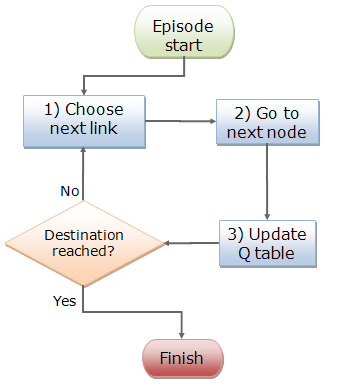
\includegraphics[width=7cm]{img/flowchart2.png}}
    \caption{RL for route choice algorithm flowchart}
    \label{fig:flowchart}
\end{figure}
%TODO discuss hypothetic distribution on the text

At step 1 drivers choose an outbound link to traverse according to the $\epsilon$-greedy action selection strategy: choose an arbitrary link with probability $\epsilon$, or choose the best link according to the Q-table with probability $1-\epsilon$. At step 2, drivers reach the destination of the chosen link and experience their travel times given by Eq. \eqref{eq:tt}.

% given by Eq. \eqref{eq:att}, where $\att{i}$ is the travel time experienced by driver $i$ and $\travTime$ is the travel time function (Eq. \eqref{eq:tt}) with $\veh$ being the number of drivers on link $l$.
%TODO realocate actual travel-time equation
% \begin{equation}
% \label{eq:att}
% \att{i} = \sum_{l \in \route{i}} \travTime(\veh)
% \end{equation}

Then, at step 3, drivers update their Q-tables using the Q-learning update formula (Eq. \eqref{eq:qlearning}), where $Q(a)$ is the Q-value for action `choosing link $a$', $\alpha$ is the learning factor, $\gamma$ is the discount factor and $R$ is the reward received by the driver for traversing link $a$.

\begin{equation}
\label{eq:qlearning}
Q(a) = (1 - \alpha) Q(a) + \alpha (R + \gamma max(Q(a')))
\end{equation}

%TODO explain why only Q(a) instead of Q(s,a) // just adopt Q(s,a) ...?

Step 4 tests whether the node reached in step 2 is the driver's final destination. If so, the trip ends, otherwise steps 1 to 3 are repeated. When the trip ends, each driver $i$ calculates the travel time $\att{i}$ experienced on it's route $\route{i}$. It is given by the sum of the travel times experienced on each link of $\route{i}$. Eq. \eqref{eq:att} illustrates this, with $\veh$ being the number of vehicles on link $l$.

\begin{equation}
\label{eq:att}
\att{i} = \sum_{l \in \route{i}} \travTime(\veh)
\end{equation}

% \subsection{Reward function}
% \label{sec:reward}

% By traversing a road, a driver receive a reward $\reward{}$, defined in equation \eqref{eq:rByCombination}%, where $\reward{t}$ is the reward component regarding the travel time, $\reward{o}$ is the reward component regarding road occupation and `$s$' is a coefficient to balance the weight of each reward component.

% \begin{equation}
% \label{eq:rByCombination}
% \reward{} = s(\reward{t}) + (1 - s)(\reward{o})
% \end{equation}

%Ranging from 0 to 1, $s$ determines if the driver will try to minimize his travel time (higher values of $s$) choose roads with less occupation (lower values of $s$).

%The component regarding the travel time ($\reward{t}$) is given by equation \eqref{eq:rByTravelTime}, where $t_l(v)$ is the travel time function given by equation \eqref{eq:tt} with $v$ being the number of drivers on link $l$.

% \begin{equation}
% \label{eq:rByTravelTime}
% R_t = - t_l(v)
% \end{equation}

%Where $at_P$ is the actual travel time experienced by the driver (eq. \eqref{eq:att}) and $et_{P^*}$ is the expected travel time for the driver (eq. \eqref{eq:ett}). The purpose of the route weight is to make the driver avoid apparently good links which result in bad options in subsequent decisions.

% In this component, the reward decreases as travel time increases. This is to foster drivers to choose routes which will result in smaller travel times. By using this component (higher values of $s$ on \eqref{eq:rByCombination}), it is expected that drivers try to minimize individual travel times, making selfish choices. That is, if a congested link or route leads to the final destination faster than uncongested alternative, they are expected to choose the congested option. 
% 
% The reward component regarding road occupation ($R_o$) is given by equation \eqref{eq:rByRoadOcc}, where $c_l$ is the capacity of link $l$ and $v$ is the number of vehicles on this link.
% 
% \begin{equation}
% \label{eq:rByRoadOcc}
% R_o = \left(\frac{c_l}{v}\right) - 1
% \end{equation}
% 
% This reward component will become positive if drivers choose an uncongested link ($c_a > x_a$) and will become negative if the number of vehicles on the link becomes higher than it's capacity. By using this component (smaller values of $s$ on \eqref{eq:rByCombination}), it is expected that drivers make choices in order to avoid congestion and alleviate the traffic flow on the network, even if it result in higher individual travel times.

\subsection{Evaluation metrics}

\subsubsection{Reasonable travel times:}
In Section \ref{sec:intro}, it was said that actual travel times experienced by the drivers can be considered reasonable when they are within the expected travel time.

In a real world situation, drivers have an expectation on the travel time needed to reach their destinations based on the route length and the expected number of drivers in it. In the present work, for each driver $i$, the expected travel time $\ett{i}$ on his optimal route \optRoute{i} is given by Eq. \eqref{eq:ett}, where $\travTime$ is the travel time function defined in Eq. \eqref{eq:tt} applied to the estimated number of vehicles on the same route ($\expVeh$). This estimation is given by the number of vehicles in driver $i$ OD pair, plus a random number in the range [-50:50]. This ``noise'' is to simulate the effect of each driver ``guessing'' the number of vehicles going to the same destination.

\begin{equation}
\label{eq:ett}
\ett{i} = \sum_{l \in \optRoute{i}}\travTime(\expVeh)
\end{equation}

In order to assess how reasonable are the travel time obtained by drivers using the proposed algorithm, a metric called AED was created. It is given by the average of the difference between actual and expected travel times achieved by the drivers of a given OD pair. For this metric, negative values are desired as this means that actual travel times are lower than the expected by the drivers.

\subsubsection{Road network load balance:}

From a global point of view, it is desired that vehicles get distributed proportionally to the capacity of each road on the network. %In the present work, vehicle distribution over the network emerges from individual decisions that each driver make using the RL for route choice algorithm. 
Road network load balance will be measured in two forms: number of congested roads ($n$) and overload factor ($o$). Considering C as the set of congested roads, these metrics will be measured according to Eq. \eqref{eq:balanceMetrics}, where $\veh_l$ and $\linkCap$ are the number of vehicles and the capacity of link $l$, respectively. 

\begin{equation}
\label{eq:balanceMetrics}
\numCong = |\congRoads| \hspace{1.5cm}  \overLoadFactor = \sum_{l \in \congRoads} \left(\frac{\veh_l}{\linkCap} -1 \right)
\end{equation}

The two metrics are needed because the number of congested roads does not measures how heavy are the roads congestions and the overload factor does not shows whether there are multiple roads slightly overloaded or just few heavily overloaded. For both ($n$) and ($o$), smaller values means better performance, as less roads are congested and the severity of congestions is lower.

\subsection{Studied scenario}

The abstract road network used in the present work is the same used by \cite{Galib&Moser2011}. It consists on 10 nodes and 24 links, as depicted in Figure \ref{fig:roadnetwork}. All nodes have 3 outbound links, except nodes 8, 9 and 10 which have 2, 1 and 0 outbound links, respectively. Nodes 1, 2 and 3 are the possible origins and nodes 8, 9 and 10 are the possible destinations, resulting in nine possible OD pairs. The network links have the same weights, representing no differences on their lengths.

\begin{figure}[ht]
    \centerline{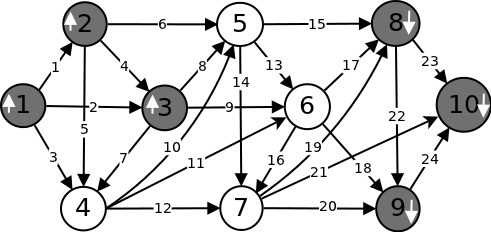
\includegraphics[width=8.5cm]{img/roadnetwork.png}}
    \caption{Road network, the same used by \cite{Galib&Moser2011}. Labels on links are identification numbers, nodes with upward arrows are the origins and downward arrows represent the destinations}
    \label{fig:roadnetwork}
\end{figure}

The proposed algorithm will be compared with three different approaches:

\begin{itemize}
  \item Random: At each step, drivers choose one of the possible outbound links with random probability.
  \item Greedy: At initialization, the shortest paths\footnote{It is possible to have more than one shortest path on the road network. Given that link's weights are equal, the shortest paths will be the ones with less links.} for each driver are calculated. At each step, drivers choose one of the possible outbound links with a probability proportional to its capacity. The possible outbound links are the ones that belongs to a shortest path.
  \item Minority Game: In this approach, drivers use a modified minority game algorithm to build their routes. For a complete description of the algorithm, it is suggested that readers refer to \cite{Galib&Moser2011}.
\end{itemize}

\section{Results and discussion}
\label{sec:results}

In the experiments, the link's capacities were randomly assigned within the range [130:250] prior to the simulations. The values are persisted from one simulation to another to ensure a correct comparison of different algorithms. The same is done for the amount of drivers on each OD pair. There are 1001 drivers on the road network. For the travel time equation \eqref{eq:tt}, the
constant $\fftt$ is set as 5 minutes for all links. The parameters  $\tau$ and $\beta$ are set as $1$ and $2$, respectively. This means that, as the number of drivers on a link increases, the travel time increases quadratically. 

\subsection{Influence of Q-learning parameters}

Several simulations were run to assess the effect of Q-learning parameters, namely the learning rate ($\alpha$) and the discount rate for future rewards ($\gamma$).

\begin{figure}[ht]
  \centering
  \subfigure[]{
    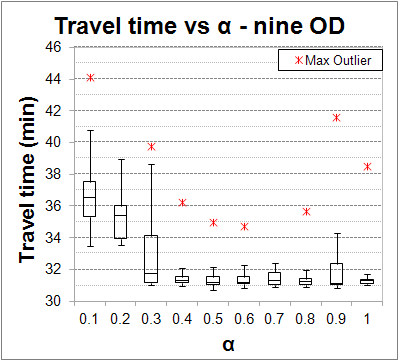
\includegraphics[width=9cm]{img/travelTimeVsAlpha.png}
    \label{fig:travelTimeVsAlpha}
  }
  \subfigure[]{
    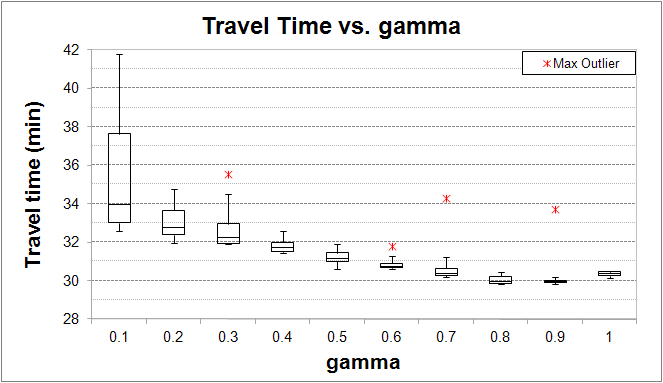
\includegraphics[width=9cm]{img/travelTimeVsGamma.png}
    \label{fig:travelTimeVsGamma}
  }
  \caption{Box-and-whisker charts showing the effect $\alpha$ and $\gamma$ on travel time. Each parameter value was tested 10 times.}
  \label{fig:qLearningParams}
\end{figure}

Figure \ref{fig:qLearningParams} shows that for $\alpha$ within the range of 0.4 to 0.8, travel time does not change in a significant way. On Fig. \ref{fig:travelTimeVsGamma}, a decrease on travel time is observed with the increase of $\gamma$. These plots shows that a good choice for the parameters are $\alpha = 0.5$ and $\gamma = 0.9$, as lower travel times are achieved with these values. They will be used for the experiments that follows.

\subsection{Comparison with other algorithms}

For each algorithm, the AED (actual and expected travel time difference) is shown on Figure \ref{fig:travelTimeComparison}. 

\begin{figure}[ht]
    \centerline{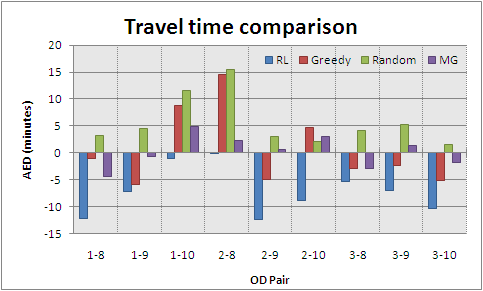
\includegraphics[width=8.5cm]{img/travelTimeComparison.png}}
    \caption{AED metric comparison for each algorithm. RL and MG are the reinforcement learning and minority game approaches, respectively}
    \label{fig:travelTimeComparison}
\end{figure}

In this metric, the RL approach outperforms the others, achieving reasonable travel times in all OD Pairs. The minority game algorithm achieves travel times within expectation in 4 OD pairs. On the other OD pairs, the performance is still good, as actual travel times are no longer than 5 minutes beyond the expected, showing a degree of fairness of the algorithm. With the greedy approach, drivers from 5 OD pairs experience travel times within expectation, but especially on OD pairs 1-10 and 2-8, actual travel times are far beyond the expected. The worst approach is the random, in which no drivers achieve reasonable travel times.


On the defined load balance evaluation metrics, the minority game based approach achieved the best results. Both the number of congested roads and the overload factor (which is based on the sum of congested roads occupation) were the lowest. This means that vehicles were distributed over the network in a proportion that is closer to the roads capacity. The RL based algorithm achieves good results. %The overload factor in this case shows that no road got

\begin{figure}[ht]
    \centerline{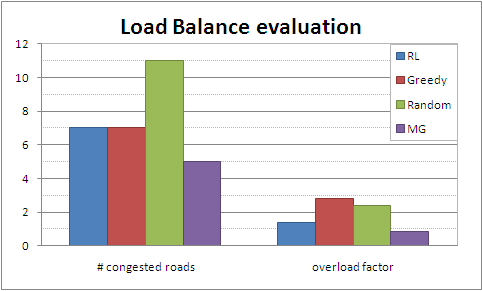
\includegraphics[width=8.5cm]{img/loadBalance.png}}
    \caption{Load balance evaluation in terms of number of congested roads and the overload factor}
    \label{fig:loadBalance}
\end{figure}




\section{Conclusions and future work}
\label{sec:conclusions}

In this work we presented a new algorithm for route choice in an abstract traffic scenario using reinforcement learning. Our approach is helpful for either individual and global point of view, as drivers achieve reasonable travel times, on average, and only few roads are overused.

Nevertheless, the proposed approach is based on realistic assumptions as it only relies on drivers own experience about the road network, dismissing the use of real-time information and historic data of roads. This makes our algorithm an attractive alternative to be used on existing navigation systems, as no new technologies are required.

This work is an successful application of the independent learners concept on a complex, competitive scenario. Agents learned how to choose routes to their destinations even considering other agents as part of the environment.

Further investigation can be conducted to assess how the algorithm performs in heterogeneous scenarios, that is, when there are drivers who use other decision processes or algorithms. Future works can also attempt to assess how good it would be for agents when they consider other agents on the environment, that is, how good it would be to learn joint actions in this competitive environment.

\bibliographystyle{splncs03}
\bibliography{references,stringDefs,AB,CD,EG,HJ,KL,MO,OURS,PR,S,TZ} 

\end{document}
